\documentclass[9pt,journal,a4]{IEEEtran}

\usepackage{cite}
\usepackage{amsmath}
\usepackage{graphicx}
\usepackage{textcomp}
\usepackage{color}
\usepackage{soul}
\usepackage{booktabs}
\graphicspath{{figures/}}

\begin{document}

\title{From Individual Uncertainty to Collective Predictability: The Impact of Temporal and Population Aggregation on Temperature-Driven Thermostatic Loads}


\author{Alexandre~M.~V.~Gouveia}

\maketitle

\begin{abstract}
Electric Thermostatic Loads (ETLs) place temperature-correlated demand on low-voltage (LV) networks, yet a Distribution System Operator (DSO) meters only aggregated net load and rarely the number of consumers behind it. This paper fits a piecewise-linear temperature response to aggregated LV net load and derives from it three quantities a DSO can act on: the temperature-driven energy ETLs consume, their installed capacity and the flexibility their coincidence implies. Consumer aggregation is treated as the variable governing which of these is identifiable, separating the predictability it confers from the attributability it removes. The fit sharpens with the consumer count and the averaging window, as expected of an aggregated LV load. The fitted Simultaneity Factor is found invariant to ETL penetration and to installed power within a population, so a curve fitted on submetered substations transfers to un-submetered ones of the same population without loss of accuracy. Installed capacity is estimated by a regression calibrated on submetered substations and, alternatively, by dividing the observed coincident peak by the transferred Simultaneity Factor. Both the fit and the coincidence transfer are validated on a real out-of-sample feeder, where installed capacity is recovered to within a few percent, and to single digits without any local submetering. The aggregation effect is reproduced on two further datasets from different climates, one driven by cooling rather than heating.
\end{abstract}

\begin{IEEEkeywords}
Electric thermostatic loads, heat pumps, low-voltage networks, degree-day regression, smart meter data, distribution system observability.
\end{IEEEkeywords}


\section{Introduction}

\begin{itemize}

\item \textbf{Macro driver.}

Electrification of heating and cooling, driven by decarbonisation policy.


\item \textbf{Concession then problem.}

Electric Thermostatic Load (ETL) uptake is a positive driver for decarbonisation, yet introduces temperature-correlated demand on low-voltage (LV) networks not sized for it.


\item \textbf{Narrow to the gap.}

Distribution System Operators (DSOs) hold net-load and weather data at the substation, and the thermal response of an ETL population is in principle visible in it. What is generally absent is the context needed to interpret that response: appliance registers, nameplate ratings and, critically, the number of consumers the substation serves. Concrete figures on registry coverage should be provided here.

The aggregation level is consequently not a fixed property of the problem but an unknown that varies between substations, and it governs both how clearly the thermal response appears and how ambiguous its origin is.


\item \textbf{Literature in named categories.}

The relevant literature should be organised into the following categories:

\begin{itemize}

\item Load Disaggregation;

\item Change-Point and Degree-Day Regression;

\item Installed-Capacity Estimation of Behind-the-Meter assets; and

\item Diversity and Simultaneity in Network Planning.

\end{itemize}

A non-exhaustive summary table of prior work should also be included.


\item \textbf{Gap, contributions, and roadmap.}

Previous work establishes the load--temperature relationship using submetered thermal load, where the thermal contribution is directly observable, or at a single fixed level of aggregation. The aggregation level itself has not been treated as the variable that governs what remains identifiable.

This paper makes the following contributions:

\begin{enumerate}

\item It formalises consumer aggregation as the governing variable in the identifiability of Electric Thermostatic Loads from aggregated LV net load, separating the predictability that aggregation confers from the attributability it removes.

\item It derives three use cases from a single temperature-response fit, namely temperature-driven Energy Forecasting, Installed-Capacity Estimation and Flexibility characterisation, and reports each against the aggregation level. Each is scored against submetered ground truth, yet requires only net load and ambient temperature to run.

\item It shows that the fitted Simultaneity Factor is invariant to ETL penetration and to installed power within a population, and that a Simultaneity Factor fitted on submetered substations transfers to un-submetered substations of the same population without loss of accuracy.

\item It estimates installed ETL capacity from net load by two routes, a regression calibrated on submetered substations and the transferred Simultaneity Factor, and compares their accuracy and their transfer to an unseen population.

\item It validates the fit, the capacity estimate and the coincidence transfer on a real, physically aggregated feeder held out of sample, and reproduces the aggregation effect on two further datasets from different climates and building stocks, one driven by cooling rather than heating.

\end{enumerate}

\item \textbf{Roadmap.}

The rest of the paper is structured as follows: Section~\ref{section:identify} formalises the thermal response of aggregated net load and the two opposing effects of consumer aggregation; Section~\ref{section:aggregation} describes the data and the substation designs, and reports how the fit and the Simultaneity Factor respond to aggregation, including how the Simultaneity Factor transfers within a population; Section~\ref{section:usecases} implements the three use cases against the aggregation level; Section~\ref{section:validation} validates the fit and the capacity estimate on a real out-of-sample feeder; in Section~\ref{section:discussion}, accuracy, generalisability, data requirements and interpretability are discussed. Lastly, Section~\ref{section:conclusion} concludes the paper.

\end{itemize}

\section{Aggregation and the Identifiability of Thermal Loads}
\label{section:identify}

In this section, the thermal response of aggregated LV net load is formalised. Consumer aggregation is then shown to act on this response in two opposing directions, and the use cases implemented in the remainder of this paper follow from the tension between them.


\subsection{Thermal Response of Aggregated Net Load}

ETLs, a class comprising heat pumps, direct resistive heating and electric cooling, modulate their electrical consumption in response to ambient temperature. At the individual consumer level this behaviour is thermostatically controlled and strongly intermittent: a single ETL is either running or idle, and its instantaneous demand is a poor indicator of the temperature that caused it. Aggregation over the consumers downstream of an LV substation removes that intermittency. Thermostatic cycling decorrelates between dwellings and idiosyncratic occupancy averages out, so the aggregate response becomes smooth and approximately piecewise linear in temperature.

The model below is therefore a description of a population rather than of a consumer, and the size of that population is a condition for the model to hold at all rather than an incidental detail.

Aggregated net load is modelled as
\begin{equation}
P(T)
=
P_{\mathrm{base}}
+
s_h \max\left(0,T_h-T\right)
+
s_c \max\left(0,T-T_c\right),
\label{eq:thermal-response}
\end{equation}
where $P$ is the aggregated net load [kW], $T$ is the ambient temperature [$^\circ$C], $P_{\mathrm{base}}$ is the temperature-independent component [kW], $s_h$ and $s_c$ are the heating and cooling Thermal Sensitivities [kW/$^\circ$C], and $T_h$ and $T_c$ are the corresponding threshold temperatures [$^\circ$C]. The interval $[T_h,T_c]$ is a dead band over which no thermal response is present, with $T_h \leq T_c$ imposed during fitting. The $\max\left(0,T_h-T\right)$ and $\max\left(0,T-T_c\right)$ terms are also called Heating Degrees (HD) and Cooling Degrees (CD), respectively.

Equation~\eqref{eq:thermal-response} describes a V-Shaped Fit. Where no electric cooling is installed, $s_c$ is zero, and the expression reduces to a Hockey-Stick Fit observed in low temperatures. Similarly, when no electric heating is present, $s_h$ is zero, and only the cooling portion of the fit is observed.

Fig.~\ref{fig:bathtub} shows the full V-Shaped form recovered from measured data, on an aggregate of 22 air-conditioned dwellings in Austin, Texas. Both arms and the intervening dead band are present: a heating sensitivity of 0.68~kW/$^\circ$C below $T_h = 11.2^\circ$C, a cooling sensitivity of 3.05~kW/$^\circ$C above $T_c = 19.8^\circ$C, and a flat interval between the two.

The two arms are not produced by the same device, and only one of them is an ETL. Circuit-level submetering attributes the cooling arm to the air conditioners, whereas 21 of the 22 dwellings draw essentially nothing on that circuit in winter. The heating arm comes instead from the furnace circuits, which the dataset defines as furnace and air handler combined, at a median 0.08~kW per dwelling in cold weather. No dwelling in the pool carries a dedicated electric heater circuit and gas service is recorded for most, so that draw is an air handler rather than electric resistance heat, and the heat itself never reaches the electricity meter. Equation~\eqref{eq:thermal-response} describes the aggregate response in either case, which is what the figure is shown for, though the distinction matters wherever an arm is read as evidence of an ETL.

\begin{figure}[t]
\centering
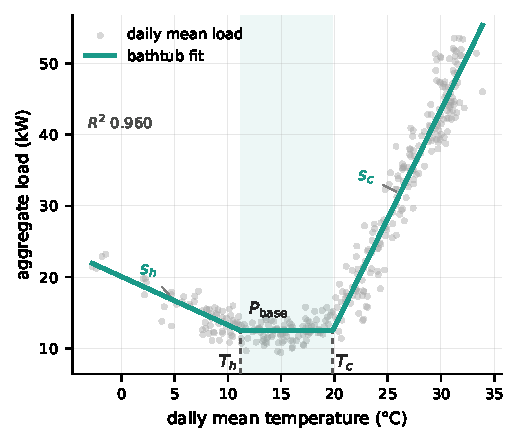
\includegraphics[width=\columnwidth]{figures/fig_bathtub_example.pdf}
\caption{Equation~\eqref{eq:thermal-response} fitted to an aggregate of 22 air-conditioned dwellings in Austin, Texas, over calendar year 2018. The parameters are marked on the curve: the base load $P_{\mathrm{base}}$, the heating and cooling thresholds $T_h$ and $T_c$ bounding the dead band (shaded), and the heating and cooling slopes $s_h$ and $s_c$.}
\label{fig:bathtub}
\end{figure}

\subsection{The Two Effects of Consumer Aggregation}
\label{subsection:two-effects}

The first effect of increasing the consumer count $N$ is to improve how well Equation~\eqref{eq:thermal-response} describes the data. Averaging over more consumers suppresses the idiosyncratic component of demand while leaving the temperature-driven component intact, since only the latter is common to every consumer downstream of the substation. The fitted parameters are correspondingly better determined. Section~\ref{section:aggregation} quantifies the improvement in the fit and in the spread of the parameters alike, and in each the gain is largest where ETL penetration is lowest.

The second effect runs the other way. The aggregated sensitivity is the sum of the individual sensitivities of all consumers downstream of the substation, and consumers without an ETL are not thermally inert. Lighting and occupancy patterns correlate with the seasonal temperature cycle, so a small positive per-consumer sensitivity remains even in the absence of ETLs. This residual term is more than an order of magnitude smaller than that of an ETL, yet it accumulates with substation size. A large ETL-free substation can therefore slope as steeply as a small ETL-bearing one, so a given heating sensitivity is consistent with many combinations of consumer count and ETL count, neither of which the DSO generally knows. Aggregation buys a better-determined curve at the cost of a more ambiguous one.

The obstruction is not a large consumer count but an unknown one: were the count published alongside the aggregated consumption, the non-ETL contribution could be subtracted and the ambiguity would not arise. This split of the aggregated slope into a non-ETL and an ETL part is set out in Section~\ref{subsection:accuracy}, where it explains where the use cases lose accuracy rather than being pursued as a result in itself.

Aggregation over time acts on the same trade-off, and for the same reason. Fitting is performed on daily aggregates rather than at the native measurement resolution, since averaging over a full diurnal cycle removes occupancy-driven variability that is not temperature-dependent. It also removes the effect of buildings' thermal inertia, which causes a mismatch between consumption and outdoor temperature at high resolutions. This averaging comes at the cost of intra-day detail. Consumer count and averaging window are two axes of one operation, and Section~\ref{section:aggregation} reports the fit against both.


\subsection{Identifiable Quantities and Use Cases}

The parameters of Equation~\eqref{eq:thermal-response} support three use cases. They differ in whether they read the fit alone or combine it with the coincidence of the population, and in how much of the aggregation level each needs to be known.

\textbf{Energy Forecasting.} Integrating Equation~\eqref{eq:thermal-response} over the temperature profile of a given day yields the temperature-driven energy consumed on that day. Driven by a forecast temperature rather than a measured one, the same integral forecasts the next day's ETL energy. For the heating arm, this reduces to the product of $s_h$, the HD value of that day, and the number of hours over which it applies. The cooling arm follows from the equivalent product using CD. The estimate refers to the total temperature-driven energy, since the non-ETL consumers contribute to it alongside the ETLs, and isolating the ETL share means removing that non-ETL contribution, discussed in Section~\ref{subsection:accuracy}. The dead band bounds where the estimate can be accurate at all: above $T_h$ the thermal term is identically zero, so any ETL energy that persists into mild weather is unexplained by construction, not by a fitting failure. Section~\ref{subsection:energy} checks accuracy against both ETL penetration and the observed temperature range accordingly.

\textbf{Installed-Capacity Estimation.} The installed capacity of an ETL population is the sum of the individual rated powers, a non-coincident quantity the net load does not observe directly. What the fit observes is the coincident peak, the aggregate ETL demand at the coldest temperature, given by the heating term of Equation~\eqref{eq:thermal-response} at that temperature. The ratio between the two is the coincidence of the population, so the coincident peak recovers the installed capacity once that coincidence is known. Section~\ref{subsection:capacity} supplies the coincidence by two routes, a regression calibrated on submetered substations and the Simultaneity Factor of Section~\ref{subsection:simultaneity}, neither of which is read from a single substation's net load alone.

\textbf{Flexibility Characterisation.} The same coincidence bounds the flexibility a heat pump population offers. The gap between the installed capacity and the coincident demand is load that is connected but not drawn at once, and the Simultaneity Factor is the fraction that is. Section~\ref{subsection:flexibility} reads this as a flexibility envelope, qualitatively, since its magnitude in kilowatts follows from the installed capacity of Section~\ref{subsection:capacity} rather than from the fit alone.

The three use cases are consequently reported against the aggregation level in Section~\ref{section:usecases}, rather than at a single one. Energy Forecasting reads the fit directly. Installed-Capacity Estimation and Flexibility Characterisation additionally require the coincidence of the population, which is why the Simultaneity Factor of Section~\ref{subsection:simultaneity} and its transfer are established before either is implemented.


\section{Aggregation and Predictability}
\label{section:aggregation}
In this section, the first of the two effects described in Section~\ref{subsection:two-effects} is measured. The datasets and substation designs are described first. Fit quality is then reported against consumer count on the training data, and reproduced on two further datasets drawn from different climates and building stocks.


\subsection{Datasets}
\label{subsection:data}

The training data is the HEAPO dataset, complemented with additional smart-meter data providing submetered thermal load. Both are Swiss, and together give net load at 15-minute resolution for 1702 LV consumers over calendar year 2023. Of these, 395 have an ETL, of which 81 carry a submetered heat pump. Heat pumps are the only ETL used in this paper, since they are the only ETL technology with a submetered thermal series in either dataset: the heat pump is the only device paired to a household meter in this data. The remaining 314 ETL-equipped consumers are identified from survey flags alone and are not used in the substation designs below. Ambient temperature is available hourly, which sets 1~h as the finest resolution at which the fit is evaluated.

A consumer is classified as ETL-free where it carries no submetered heat pump and none of five labelled electric heating types is recorded in the household survey: electric water heater, storage heating, direct heating, auxiliary heat pump and water-heating heat pump. This leaves 1307 ETL-free consumers. The negative class is therefore defined rather than filtered, which a heat-pump-specific framing would not achieve, since a consumer with resistive heating would remain in the reference group and contaminate it.

The validation data is WPUQ, 37 German single-family houses on one low-voltage feeder, each with separately metered heat pump and household circuits, over calendar year 2019. Ambient temperature is recorded at five-minute resolution against the training data's hourly series, though every fit in this paper rests on hourly temperature at the coarsest, so the difference does not propagate into the results. The data predates the German regulatory provisions for controllable heat pump loads that came into force in 2024.

A third dataset supplies the cooling arm, which neither of the others contains. Pecan Street's Austin panel gives 22 air-conditioned dwellings in Texas over calendar year 2018 at 15-minute resolution, each with circuit-level submetering. Its air conditioners are a genuine ETL and dominate the summer load, drawing 25~kW summed over the pool above 25$^\circ$C against 1~kW below 10$^\circ$C. Its heating arm is not an ETL, for the reason given in Section~\ref{section:identify}, so Austin is used to test the aggregation claim on a cooling-driven fit rather than to add a second heating population.

Neither Swiss nor WPUQ consumers carry a labelled cooling load, and the summer behaviour of the WPUQ heat pumps is consistent with this. Pooling its 37 units over June-August, the correlation between load and temperature is negative in 18 of 37 cases at $p<0.05$ against positive in 2, and the median correlation across all units is $-0.18$. The cooling sensitivity $s_c$ is consequently zero for both, and only the heating arm of Equation~\eqref{eq:thermal-response} is fitted on either. Austin is the one dataset where both arms are free.


\subsection{Substation Designs}
\label{subsection:designs}

Synthetic substations are drawn from the Swiss pool, each consumer appearing at most once within a given substation but reused freely across substations. Consumer count $N$ and ETL count $N_{\mathrm{etl}}$ are varied independently over a factorial grid of 12 sizes and 5 penetration levels, at 25 replicates per cell, giving 1500 substations. The five penetration levels are 0, 25, 50, 75 and 100\%, and the 0\% cells supply an ETL-free reference group, used in Section~\ref{subsection:fitquality} to show that the fit forms even where no ETL is present. Every substation is tied to a single weather station, so that one temperature series applies to all of its members. The 81 submetered heat pumps are split across stations and the largest holds 50 of them, which caps $N$ at 48 for the fully penetrated cells, where $N_{\mathrm{etl}} = N$.

The design does not exhaust the pool. Drawing is confined to one weather station per substation and stops at $N = 48$, so 1384 of the 1702 consumers and 77 of the 81 submetered heat pumps are actually used, and every figure below refers to those.

The 1500 substations are also not 1500 independent observations. They are built from those 1384 consumers, of which only the 77 carrying a submetered heat pump ever supply the ETL tier, so each of the 77 appears in approximately 250 substations. Reuse is also uneven across the grid rather than uniform. Replicates within a cell share a mean 3\% of their ETL members at $N = 4$ and 25\% penetration, against 92\% at $N = 48$ and full penetration. At that corner 48 members must be drawn from the 50 heat pumps the station holds. The design is consequently a controlled traverse of the $N \times N_{\mathrm{etl}}$ grid rather than a sample of a substation population, and the replicates suppress the variability of the draw rather than measure that of the consumer population. Intervals reported below are therefore obtained by resampling consumers rather than substations, and comparisons that hold the consumers fixed and vary something else, such as the resolution comparison of Section~\ref{subsection:resolution}, are paired and do not inherit the same difficulty.

WPUQ cannot support the same factorial design, since every household carries a heat pump, so penetration cannot be varied and no ETL-free reference group can be formed. It is used instead for the nested aggregation test below and, in full, for the real-feeder validation of Section~\ref{section:validation}.

The aggregation claim carries no such difficulty, since it concerns how the fit responds to consumer count rather than how two classes separate. It is tested on WPUQ with one substation per aggregation level, in a nested sequence: the aggregate at $N$ contains the aggregate at $N-4$. Each step is therefore the addition of four consumers to a fixed set rather than a comparison between independent draws. Roles are fixed before any aggregate is built, half the pool contributing its heat pump circuit and half having it withheld, which holds penetration at 50\% throughout and matches the condition reported for the training data below.

Nine substations result, from $N = 4$ to $N = 36$. No replicates are drawn and none are implied. A factorial design over the same 37 houses would yield a larger substation count without a corresponding gain in evidence, for the reason just given. The single nested sequence instead makes the dependence on $N$ visible without inviting a precision claim the pool cannot support.

Austin is aggregated the same way, in a nested sequence from $N = 4$ to $N = 22$ in steps of two. There is no penetration to hold fixed, since every dwelling in the pool has an air conditioner, so each level is simply the first $N$ of one fixed random ordering. Both arms of Equation~\eqref{eq:thermal-response} are fitted at every level.

Every result on the training data is evaluated on the same calendar year the parameters were fitted on, with no held-out period. This is not a like-for-like restatement of the fit, since the fit target is net load throughout, whereas Energy Forecasting is scored against submetered thermal energy the fit never sees. It does mean those figures carry no penalty for temporal extrapolation. WPUQ supplies the genuinely out-of-sample test, on a dataset from a different year, country and building stock.

Network losses between the consumers and the substation are neglected. However, since the objective is to obtain realistic substations rather than exact recreations of a particular network, this assumption is reasonable. The WPUQ feeder carries a measured transformer against which the synthetic aggregation can be checked directly. Its 37 monitored households account for 49.5\% of the transformer's mean load and the two series correlate at 0.95, so the monitored set behaves as a substantial and representative fraction of a real feeder.


\subsection{Fit Quality Against Aggregation Level}
\label{subsection:fitquality}

That aggregation improves the fit is expected, and well established for LV load in general, the more so for spatial aggregation, where more consumers make the aggregate more predictable. It is reported here as the condition the later use cases rest on, rather than as a result in its own right. The value added below is which quantities the improving fit makes identifiable, and at what aggregation level each becomes usable.

The effect is directly observable on the training data. Median net-load $R^2$ at 24~h rises with the consumer count at every penetration level: from 0.710 at $N = 4$ to 0.921 at $N = 48$ for substations at 25\% penetration, and from 0.856 to 0.948 at 50\%. The gain is largest where the ETL signal is weakest. At full penetration the same range yields only 0.925 to 0.958, since the response is already well determined by the ETLs alone.

The ETL-free reference group shows the effect in isolation. Substations carrying no ETL reach a median $R^2$ of 0.188 at $N = 4$ against 0.524 at $N = 48$, so aggregation renders identifiable a temperature response that no ETL produces. This is the non-ETL response of Section~\ref{subsection:two-effects} becoming a well-determined curve in its own right, quantified later in Section~\ref{subsection:accuracy}, and it is why the quality of a fit is not by itself evidence of an ETL.

The fitted parameters stabilise alongside the fit. The relative interquartile spread of $s_h$ across the replicates of a cell falls from 0.365 to 0.223 between $N = 4$ and $N = 48$ at 25\% penetration, and from 0.368 to 0.122 at 50\%. The corresponding figures at higher penetration are not reported here, since replicates there are drawn from a nearly exhausted pool and agree with one another for the reason given in Section~\ref{subsection:designs}, rather than because the estimate has converged.

Fig.~\ref{fig:aggregation-quality} places the consumer axis alongside the temporal one, at a fixed 50\% penetration. Both act in the same direction, which is what justifies treating consumer count and averaging window as two forms of one operation rather than as unrelated design choices. They are also partly interchangeable. Raising the consumer count from 4 to 48 gains 0.410 in $R^2$ at 1~h resolution, against 0.092 at 24~h, so much of what aggregating consumers achieves has already been achieved by averaging over time. Over part of their range the two are consequently substitutes rather than independent improvements, an interaction Section~\ref{subsection:reproduction} finds holds in one further dataset but not the other. Section~\ref{subsection:resolution} returns to the cost attached to the temporal axis.

\begin{figure}[t]
\centering
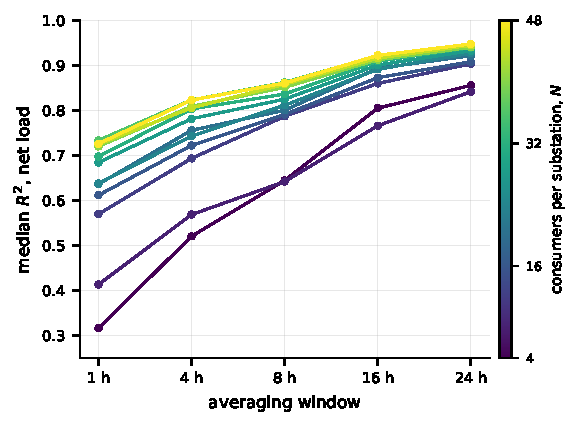
\includegraphics[width=\columnwidth]{figures/fig_aggregation_quality.pdf}
\caption{Median net-load $R^2$ against averaging window, one line per consumer count, at a fixed 50\% ETL penetration. Both aggregation axes act in the same direction, and they partly substitute for one another: the spread between consumer counts narrows as the averaging window widens.}
\label{fig:aggregation-quality}
\end{figure}


\subsection{Reproduction on Independent Datasets}
\label{subsection:reproduction}

Fit quality rises with the consumer count at every averaging window in WPUQ as well (Fig.~\ref{fig:nested-aggregation}, left). At 24~h, net-load $R^2$ goes from 0.667 at $N = 4$ to 0.845 at $N = 36$, and at 1~h from 0.499 to 0.605. The direction is the same on a dataset the fitting procedure has never seen, with no recalibration of bounds and no adjustment to the fit.

\begin{figure*}[t]
\centering
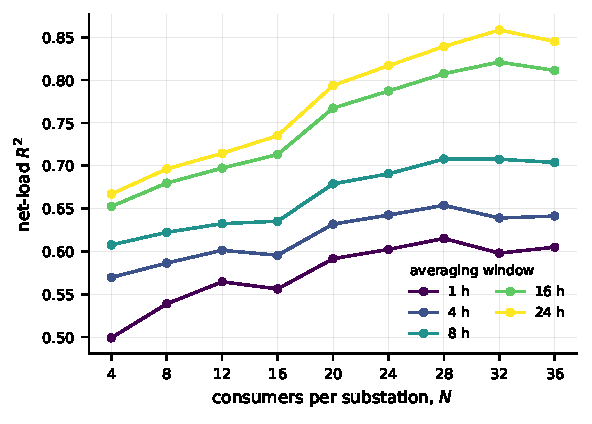
\includegraphics[width=\textwidth]{figures/fig_nested_aggregation.pdf}
\caption{Net-load $R^2$ against averaging window for the two nested sequences, one line per consumer count, drawn on the axes of Fig.~\ref{fig:aggregation-quality}. Left: WPUQ, heating arm only, at 50\% ETL penetration. Right: Austin, both arms of Equation~\eqref{eq:thermal-response} free. Each aggregate contains the one below it, so a lighter line is a strict superset of a darker one. No band is shown because there are no replicates.}
\label{fig:nested-aggregation}
\end{figure*}

Austin reproduces the same direction with both arms free (Fig.~\ref{fig:nested-aggregation}, right). Net-load $R^2$ at 24~h rises from 0.799 at $N = 4$ to 0.958 at $N = 22$, increasing at every step but a negligible dip at $N = 18$. The gain is steepest below $N = 10$ and the curve is nearly flat beyond, so most of what aggregation offers is obtained within the first dozen consumers. Reading across consumer counts rather than along the window, the rise is not strictly monotone in either dataset, which is expected of single realisations. An individual consumer added at one step may be less regular than the aggregate it joins, an irregularity the training data averages away over its replicates.

The figures also make the two-axis interaction visible, as the degree to which the lines converge from left to right. In the training data the consumer-count effect shrinks as the window widens, from 0.410 in $R^2$ at 1~h to 0.092 at 24~h, so the lines fan in and the two axes act as substitutes. Austin behaves the same way, the consumer-count effect falling from 0.261 to 0.159 over the same range. WPUQ is the exception: there the effect grows, from 0.106 to 0.178, and the lines fan out rather than in. The substitution therefore holds in two datasets of three. Its failure in WPUQ might indicate that those fits remain limited at fine resolution by something other than consumer count, its individually metered single-family houses having sharper sub-daily swings than a mixed consumer pool.

The two arms of the Austin fit do not sharpen at the same rate, which is instructive. The cooling threshold $T_c$, belonging to the air conditioners, settles at 19.8$^\circ$C and varies by a standard deviation of 0.10$^\circ$C once $N \geq 10$. The heating threshold $T_h$, belonging to no thermostatic load at all, wanders between 10.1 and 11.3$^\circ$C over the same range, at a standard deviation of 0.51$^\circ$C. Aggregation sharpens the parameter describing a real thermostatic population and leaves the other loose, which is the same asymmetry the reference group of Section~\ref{subsection:fitquality} shows from the opposite direction.

Aggregation therefore confers predictability regardless of dataset, climate, building stock or thermostatic technology.

\subsection{Coincidence of the Heat Pump Population and its Transfer}
\label{subsection:simultaneity}

A third quantity follows the same transition, and it is the one aggregation is classically expected to govern. The Simultaneity Factor (SF) is the fraction of a population's connected load drawing power at once, fitted here in the same three-parameter form as the net-load response, against submetered heat pump load normalised by its installed peak. At the individual level the quantity is degenerate, since a single heat pump is either running or idle and its coincident fraction is therefore 0 or 1. Aggregation is what renders it a stable fraction of the connected load.

Fig.~\ref{fig:simultaneity} reports the fitted SF at each substation's coldest observed day, against the number of heat pumps aggregated. The median is almost flat, moving from 0.38 at a single heat pump to 0.42 by a dozen and holding there. The spread is what changes, with the interquartile range across substations narrowing from 0.162 at one heat pump to 0.007 at 48. Aggregation does not so much reveal a coincidence value as render a fixed one certain, which is the SF reading of the individual-to-collective transition the rest of this section describes.

\begin{figure}[t]
\centering
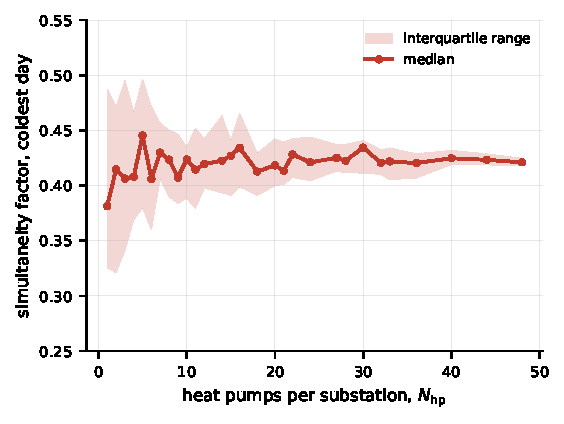
\includegraphics[width=\columnwidth]{figures/fig_sf_by_aggregation.pdf}
\caption{Fitted simultaneity factor at each substation's coldest observed day, against the number of heat pumps aggregated, on the training data. The median holds near 0.42 while the interquartile band funnels in, from 0.162 at a single heat pump to 0.007 at 48.}
\label{fig:simultaneity}
\end{figure}

The collapse is not an artefact of the replicate reuse noted in Section~\ref{subsection:designs}. Restricting to 25\% penetration, where replicates share at most 14\% of their heat pumps, the interquartile range still falls from 0.162 at one heat pump to 0.038 at twelve. The reuse only reinforces the further tightening seen at the largest counts.

The Simultaneity Factor is built from submetered heat pump load and its installed peak, neither of which a DSO holds. It is nonetheless usable on substations where nothing is submetered, because its shape transfers within a population. Fitted on one half of the substations and applied to the other, the curve reproduces the held-out Simultaneity Factor almost as well as a curve fitted on the held-out substations themselves, at a median $R^2$ of 0.965 against 0.973. The transfer holds across the whole penetration range, and survives an extreme mismatch: a curve fitted on the most penetrated third of substations reconstructs the least penetrated third to a seasonal-peak error near 6\%. A submetered pilot is therefore enough to carry the coincidence of a population onto its un-submetered substations, which Section~\ref{subsection:capacity} uses to estimate installed capacity where no heat pump is submetered.

What transfers within a population is the shape, not the absolute level. The level reflects the local climate and heat pump sizing, in the same way as the absolute Thermal Sensitivities discussed in Section~\ref{subsection:generalisability}. A curve carried to a different climate must therefore be re-read at the local balance temperature before it applies. Section~\ref{section:validation} quantifies that limit on a real German feeder. The invariance to penetration and to installed power is what makes the shape portable; the dependence on climate and sizing is what keeps its level local.

Across these readings -- fit quality, parameter spread and coincidence alike -- aggregation supplies a predictable curve whose coincidence transfers within a population. The following section turns to what that predictability is worth: the quantities the resulting fit makes identifiable, and the aggregation level at which each becomes usable.


\section{What Aggregation Makes Identifiable}
\label{section:usecases}
In this section, the three use cases introduced in Section~\ref{section:identify} are implemented. Each reads the fit whose behaviour Section~\ref{section:aggregation} established, so each is reported against the aggregation level rather than at a single one. Energy Forecasting reads the fit directly and is evaluated on the training data, for the reason given in Section~\ref{subsection:designs}. Installed-Capacity Estimation and Flexibility Characterisation additionally read the coincidence of the population, and the capacity estimate is scored on substations held out from the calibration.


\subsection{Energy Forecasting}
\label{subsection:energy}

Integrating the thermal term of Equation~\eqref{eq:thermal-response} over a day's temperature returns the temperature-driven ETL energy of that day. Driven by a forecast temperature rather than a measured one, the same term forecasts the next day's ETL energy, a quantity a DSO needs for scheduling and procurement. The estimator is validated below against measured temperature, so the accuracy reported is that of the fit rather than of the weather forecast that would drive it in operation.

Pooled across 438\,000 substation-days, the thermal term of Equation~\eqref{eq:thermal-response} reaches $R^2 = 0.953$ against submetered thermal energy, at a total-energy bias of $-11.5\%$ and a Root Mean Square Error (RMSE) of 91~kWh/day. The estimate is built from the day's mean temperature alone, and is compared against a quantity the fit never saw, since the fit target was net load rather than thermal energy.

Table~\ref{tab:energy-penetration} reports the estimator against ETL penetration. $R^2$ remains above 0.88 at every penetration level, so the forecast holds up even where the ETL share of the load is small. RMSE rises steadily with penetration, from 49~kWh/day at 25\% to 127~kWh/day at full penetration, which tracks the growing absolute scale of the substation's thermal energy rather than a loss of relative accuracy: $R^2$ does not fall over the same range.

The bias, however, changes sign. At 25\% penetration the estimator over-predicts by 1.6\%, whereas at full penetration it under-predicts by 14.5\%. This might indicate the non-ETL share of the slope becoming visible: at low penetration the non-ETL consumers contribute a larger fraction of $s_h$, so more non-ETL temperature-driven load is attributed to the ETL and the estimate is inflated accordingly, a decomposition Section~\ref{subsection:accuracy} makes explicit.

\begin{table}[t]
\centering
\caption{Energy Forecasting accuracy against ETL penetration. Bias and RMSE are total-energy statistics.}
\label{tab:energy-penetration}
\begin{tabular}{lccc}
\toprule
Penetration & $R^2$ & Bias [\%] & RMSE [kWh/day] \\
\midrule
25\%  & 0.885 & $+1.6$  & 49  \\
50\%  & 0.941 & $-9.9$  & 70  \\
75\%  & 0.947 & $-13.0$ & 97  \\
100\% & 0.949 & $-14.5$ & 127 \\
\bottomrule
\end{tabular}
\end{table}

Accuracy improves with the consumer count as well, and most visibly where penetration is lowest. Pooled over penetration, $R^2$ rises from 0.911 at $N = 4$ to 0.945 at $N = 48$. Restricting to 25\% penetration, the hardest level, the same range gives 0.668 against 0.861, and the total-energy bias falls from $+11.0\%$ to $+1.2\%$. Aggregation therefore improves both the accuracy and the calibration of the estimate precisely where the ETL share of the load is smallest.

The dispersion falls further than the median rises, which is the more consequential of the two. Fig.~\ref{fig:energy-aggregation} reports the accuracy of each substation separately rather than the median across them, at that same 25\% penetration. The interquartile range contracts from 0.470 at $N = 4$ to 0.075 at $N = 48$, against a median that moves from 0.583 to 0.885. Whether an individual four-consumer substation yields a usable energy estimate consequently depends heavily on which four consumers it happens to contain. Eight of the 300 substations at this penetration score below zero, meaning the fitted thermal term explains less than the daily mean would. By $N = 48$ that dependence has largely gone. This narrowing is not an artefact of the reuse described in Section~\ref{subsection:designs}, since replicates at 25\% penetration share at most 14\% of their ETL members at any size.

\begin{figure}[t]
\centering
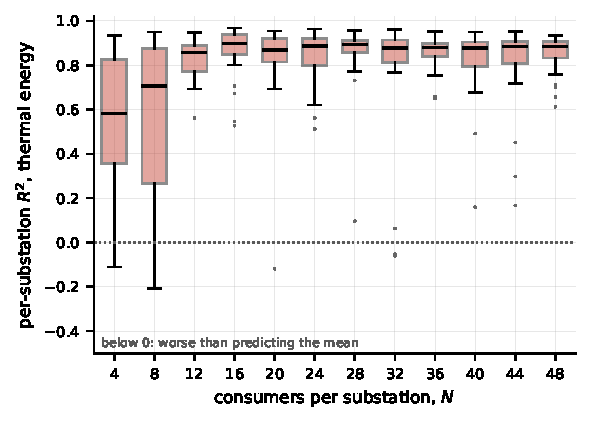
\includegraphics[width=\columnwidth]{figures/fig_energy_by_aggregation.pdf}
\caption{Per-substation accuracy of the thermal-energy estimate against consumer count, at 25\% ETL penetration. Each box holds the 25 replicates of that cell. The median rises modestly while the spread contracts sharply, so aggregation buys reliability across substations more than accuracy at the typical one. Two substations falling below the axis are not shown.}
\label{fig:energy-aggregation}
\end{figure}

The bias pooled over penetration behaves differently. It stays between $-9.9\%$ and $-12.2\%$ across the whole range of $N$, with no trend. Aggregation suppresses the variance of the estimate, and the small-sample bias that inflates it at low penetration, yet leaves the systematic shortfall untouched. That shortfall is a property of the functional form rather than of the sample, as the dead band examined below implies.

Accuracy is also not uniform across the temperature range. Splitting substation-days at the median daily mean temperature, the estimator reaches $R^2 = 0.971$ and a bias of $-2.4\%$ on cold days, against $R^2 = 0.453$ and a bias of $-54.7\%$ on warm days; RMSE is comparatively stable, at 82 and 99~kWh/day respectively. This is possibly a consequence of the dead band in Equation~\eqref{eq:thermal-response}. Above $T_h$ the thermal term is exactly zero by construction, so any ETL energy persisting into mild weather -- domestic hot water, most plausibly -- is unexplained by the estimator. A large relative bias results even where the absolute error stays modest.


\subsection{Installed-Capacity Estimation}
\label{subsection:capacity}

Installed capacity is estimated from the coincident peak the fit already observes. The heating term of Equation~\eqref{eq:thermal-response} at the coldest observed temperature gives $\delta = s_h (T_h - T_{\min})$, the aggregate ETL demand at that temperature. Capacity is the ratio of that peak to the coincidence of the population, so the two routes below differ only in how the coincidence is supplied.

The first route calibrates it. A regression of installed capacity on $\delta$ across the submetered substations returns a single coefficient, applied to $\delta$ on the substations held out. The second route reads it from the coincidence directly, dividing $\delta$ by the Simultaneity Factor transferred from the submetered substations of Section~\ref{subsection:simultaneity}. Capacity is then the coincident peak scaled by the reciprocal of the coincidence, and no capacity label is fitted.

Within the training population the calibrated regression is the more accurate (Table~\ref{tab:capacity} and Fig.~\ref{fig:capacity-scatter}), at a MAPE of 18.5\% against 23.8\% for the transferred Simultaneity Factor, and it is unbiased where the physical route over-predicts by 13\%. The difference has a single cause. The regression absorbs the non-ETL share of $\delta$ described in Section~\ref{subsection:accuracy}, whereas the Simultaneity Factor route treats the whole of $\delta$ as heat pump demand and inherits that share. The ranking reverses at high penetration, where the non-ETL share is smallest. There the transferred Simultaneity Factor is the more accurate of the two, at a MAPE of 5.9\% against 10.7\% at full penetration, since it rests on a coincidence that does not depend on the training population.

\begin{table}[t]
\centering
\caption{Installed-capacity estimation within the training population, on substations held out from the calibration. MAPE and $R^2$ are per-substation; bias is a total statistic.}
\label{tab:capacity}
\begin{tabular}{lccc}
\toprule
Route & MAPE [\%] & $R^2$ & Bias [\%] \\
\midrule
Calibrated regression & 18.5 & 0.939 & $+0.3$ \\
Transferred Simultaneity Factor & 23.8 & 0.886 & $+13.1$ \\
\bottomrule
\end{tabular}
\end{table}

\begin{figure}[t]
\centering
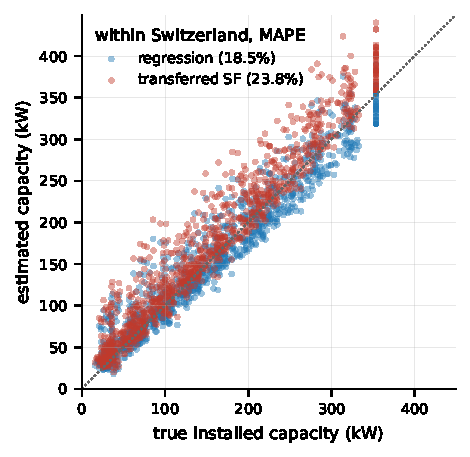
\includegraphics[width=\columnwidth]{figures/fig_capacity_scatter.pdf}
\caption{Estimated against true installed capacity on substations held out from the calibration, for the two routes. The regression lies along the identity, whereas the transferred Simultaneity Factor sits slightly above it, over-predicting by the non-ETL share of the coincident peak it does not subtract.}
\label{fig:capacity-scatter}
\end{figure}

The two routes trade places again across populations rather than within one, which Section~\ref{section:validation} takes up on the real feeder. The calibrated coefficient is tuned to the training population and transfers no better than the Simultaneity Factor whose level Section~\ref{subsection:simultaneity} shows to be local. Neither route escapes the non-ETL confound of Section~\ref{subsection:accuracy}, since both read the same $\delta$, so both under-report where the non-ETL share of the slope is large and the penetration low.

\subsection{Flexibility Characterisation}
\label{subsection:flexibility}

The Simultaneity Factor bounds the flexibility the heat pump population offers, read as the gap between the installed capacity and the coincident demand. At the coldest observed day the Swiss population draws a median fraction near 0.42 of its installed capacity. A little under three fifths of the connected heat pump power is therefore not drawn at once, and is in principle available to shift. Away from the coldest day the drawn fraction is smaller and the idle headroom larger, which the fitted Simultaneity Factor traces as a function of temperature (Fig.~\ref{fig:flexibility}).

\begin{figure}[t]
\centering
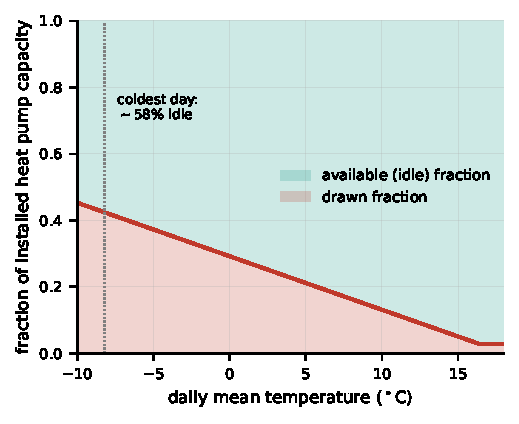
\includegraphics[width=\columnwidth]{figures/fig_flexibility_envelope.pdf}
\caption{The fitted Simultaneity Factor read as a flexibility envelope. The lower band is the fraction of installed heat pump capacity drawn at each temperature, the upper band the idle fraction available to shift. At the coldest observed day about three fifths of the connected capacity is idle.}
\label{fig:flexibility}
\end{figure}

This characterisation is qualitative. Its magnitude in kilowatts is the idle fraction multiplied by the installed capacity, so it rests on the capacity estimate of Section~\ref{subsection:capacity} and inherits that estimate's error and its confound. What the Simultaneity Factor supplies on its own, and supplies with the transferability of Section~\ref{subsection:simultaneity}, is the fraction rather than the kilowatts, so the flexibility envelope is reported as a shape against temperature and not as a firm dispatchable quantity.

\subsection{Effect of Temporal Resolution}
\label{subsection:resolution}

The daily aggregation adopted in Section~\ref{section:identify} is warranted by the fit. Net-load $R^2$ improves monotonically as the averaging window widens, reaching 0.948 at 24~h for a substation of 48 consumers at 50\% penetration, a gain of 0.22 over the 1~h fit. Total-energy accuracy is comparatively insensitive to the fitting resolution, with $R^2$ between 0.948 and 0.953 and bias between $-11\%$ and $-13\%$ across the five resolutions tested. Coarsening the window therefore improves the fit and leaves the energy forecast essentially unchanged, so neither use case calls for a finer resolution.


\section{Out-of-Sample Validation on a Real Feeder}
\label{section:validation}

The WPUQ feeder is measured as a single aggregate rather than resampled, so it validates the fit, the coincidence and the capacity estimate on a real network held out of sample. All 37 households carry a heat pump, giving a fully penetrated feeder of 238.5~kW installed capacity, well outside the Swiss training range. Its monitored households account for 49.5\% of the measured transformer load at a correlation of 0.95, as Section~\ref{subsection:designs} notes, so the aggregate stands for a substantial fraction of a real feeder rather than a contrived one.

The fit behaves as the aggregation argument predicts. On the full feeder the Simultaneity Factor is well determined, at $R^2 = 0.83$ against the 0.59 of its resampled four-pump substations, since the real feeder aggregates 37 heat pumps rather than a handful. Its fitted coincidence slope, at 0.0162 per~$^\circ$C, matches the Swiss 0.0161 almost exactly, so the coincidence physics is shared between the two populations. What differs is the balance temperature, 13.3$^\circ$C against 16.5$^\circ$C, and the milder coldest day, so the Simultaneity Factor at the coldest observed temperature is 0.32 rather than the Swiss 0.42 (Fig.~\ref{fig:real-feeder}). The German houses begin heating at a lower temperature and never reached as cold a one, so their fleet is pushed less hard, and the difference is one of climate and building stock rather than of coincidence.

\begin{figure}[t]
\centering
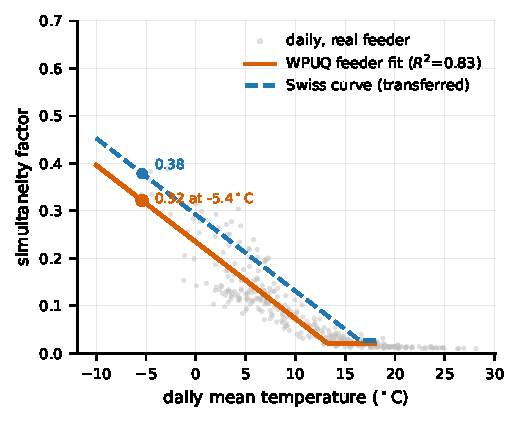
\includegraphics[width=\columnwidth]{figures/fig_real_feeder_sf.pdf}
\caption{Fitted Simultaneity Factor of the real WPUQ feeder against daily mean temperature, over all 37 heat pumps. The feeder's own fit (solid) shares the Swiss coincidence slope but a lower balance temperature, so the transferred Swiss curve (dashed) reads 0.38 at the feeder's coldest day against the feeder's own 0.32.}
\label{fig:real-feeder}
\end{figure}

The capacity estimate follows the transfer directly (Table~\ref{tab:validation}). The feeder's net-load fit gives a coincident peak of $\delta = 75$~kW. Dividing it by the feeder's own Simultaneity Factor returns 233~kW against a true 238.5~kW, an error of $-2\%$, so the coincidence route is near-exact once the coincidence is local. Borrowing the Swiss coldest-day value of 0.42 instead under-estimates by 25\%, since it is read at a temperature the feeder never reached. Evaluating the Swiss curve at the feeder's own coldest temperature, which is transferring the function rather than a single value, recovers part of that to $-17\%$. Reading the balance temperature from the feeder's own net load, an observable that needs no submetering, recovers most of the rest to $-7\%$. The residual is the coincidence slope, the one parameter of the Simultaneity Factor that a local net-load fit cannot supply, so closing it would require local submetering.

\begin{table}[t]
\centering
\caption{Installed-capacity estimation on the real WPUQ feeder (true capacity 238.5~kW), by how the Simultaneity Factor is obtained. Each row divides the same net-load coincident peak by a different Simultaneity Factor.}
\label{tab:validation}
\begin{tabular}{lcc}
\toprule
Simultaneity Factor used & SF & Error [\%] \\
\midrule
Swiss coldest-day value (constant) & 0.42 & $-25$ \\
Swiss curve at the feeder's coldest temperature & 0.38 & $-17$ \\
Swiss slope, balance temperature read locally & 0.34 & $-7$ \\
Feeder's own Simultaneity Factor & 0.32 & $-2$ \\
\bottomrule
\end{tabular}
\end{table}

The validation therefore separates what transfers from what does not, in the terms Section~\ref{subsection:simultaneity} sets out. The coincidence slope transfers across the two populations unchanged, and is the portable half of the Simultaneity Factor. The balance temperature does not, and is the half that must be read locally, which the target feeder's own net load supplies without any submetering. A capacity estimate on an unseen, un-submetered feeder is consequently accurate to single digits once the borrowed curve is re-read at the local balance temperature, and biased by a quarter if the Swiss value is transferred as a constant. The fit and the coincidence reproduce on a real network; their absolute level does not, and the correction that restores it is observable.


\section{Discussion}
\label{section:discussion}


\subsection{Accuracy}
\label{subsection:accuracy}

Accuracy improves with aggregation, though not without limit and not in every quantity. Fit quality and Energy Forecasting both rise with the consumer count, and in both cases the gain is largest where ETL penetration is lowest (Sections~\ref{subsection:fitquality} and~\ref{subsection:energy}). Aggregation is therefore most useful exactly where the ETL signal is weakest, which is the regime a DSO is likely to meet first as uptake begins. Section~\ref{subsection:reproduction} reproduces the fit-quality half of that statement on an independent dataset.

The second effect of Section~\ref{subsection:two-effects} can now be made quantitative, and it accounts for where the use cases lose accuracy. The aggregated heating sensitivity splits into a non-ETL and an ETL part,
\begin{equation}
s_h = N \sigma_{\mathrm{base}} + N_{\mathrm{etl}} \sigma_{\mathrm{etl}},
\label{eq:sensitivity-decomposition}
\end{equation}
with $N$ the consumer count, $N_{\mathrm{etl}}$ the ETL count, $\sigma_{\mathrm{base}}$ the mean per-consumer non-thermal sensitivity and $\sigma_{\mathrm{etl}}$ the mean per-ETL thermal sensitivity. A least-squares fit across the median sensitivity surface gives $\sigma_{\mathrm{base}} = 0.0054$~kW/$^\circ$C and $\sigma_{\mathrm{etl}} = 0.117$~kW/$^\circ$C, so a single ETL is worth about 22 ordinary consumers. The per-consumer term is more than an order of magnitude smaller, yet it accumulates with $N$.

This split explains the two failures the estimates share. The total-energy bias changes sign with penetration because $N \sigma_{\mathrm{base}}$ is a larger share of $s_h$ at low penetration, so non-ETL load is attributed to the ETL and the forecast is inflated. The capacity estimate under-reports at low penetration for the same reason, since both routes read a coincident peak $\delta$ that carries the non-ETL share. Pooled over penetration the total-energy bias is instead invariant to aggregation, holding between $-9.9\%$ and $-12.2\%$ across the range of $N$, since it follows from the functional form rather than the sample. Aggregation therefore improves the precision of what the fit recovers, rather than its correctness.

Installed-Capacity Estimation gains from aggregation through the Simultaneity Factor it rests on. That factor is noisy where few heat pumps are aggregated and tight where many are, so the estimate is most reliable on large feeders, as Section~\ref{section:validation} shows on a real one. Within the training population the calibrated regression reaches a MAPE of 18.5\% and the transferred Simultaneity Factor 23.8\%, the regression the more accurate because it absorbs the non-ETL share of the slope that the physical route carries through.

The clearest weakness is the accuracy of Energy Forecasting away from the coldest conditions, where $R^2$ falls from 0.971 on cold days to 0.453 on warm ones (Section~\ref{subsection:energy}). This is consistent with the dead band identified in Section~\ref{section:identify}: any ETL energy that persists above $T_h$ is unexplained by construction, not by a fitting failure, so no amount of additional data corrects it. Heat pumps commonly serve domestic hot water alongside space heating, a duty maintained throughout the year and largely independent of ambient temperature, so this share of ETL demand persists above $T_h$ regardless of season and is missed by the estimator. This marks a genuine boundary of Equation~\eqref{eq:thermal-response}, rather than a shortcoming specific to Energy Forecasting, since the fitted slope below $T_h$ is unaffected while the integral above it is not.


\subsection{Generalisability}
\label{subsection:generalisability}

Three datasets still provide a narrow basis for a general claim, though what Section~\ref{subsection:reproduction} establishes is broader than a single reproduction. The aggregation behaviour transfers: fit quality rises with the consumer count in WPUQ and in Austin as it does in Switzerland, over nested sequences in which each aggregate contains the one below it. It also survives a change of thermostatic technology, the Austin fit being driven by cooling rather than heating. The levels differ, at 0.845 against 0.948 for the largest aggregate at 24~h, and the direction does not. That the effect survives a change of country, climate, building stock and metering arrangement suggests it follows from aggregation itself rather than from anything particular to the training data.

The use cases transfer unevenly, and the differences follow from what each needs. Energy Forecasting could in principle be scored out of sample on WPUQ, yet on 37 houses from a single feeder it would rest on too narrow a base to separate a property of the method from a property of that feeder. Installed-Capacity Estimation, by contrast, is validated out of sample on that same feeder in Section~\ref{section:validation}, since its ground truth is the installed capacity the registry supplies rather than a submetered series the dataset would have to expose. A second dataset spanning more feeders would still be needed to score Energy Forecasting out of sample.

Absolute quantities are not expected to transfer in any case. Thermal Sensitivities reflect the local building stock, climate and heating practice, so recalibration at every new deployment is expected rather than a sign of failure. This is why Section~\ref{subsection:two-effects} frames its argument in terms of what aggregation does to the fit, rather than in terms of any particular fitted value.

The real-feeder result of Section~\ref{section:validation} sharpens this into a usable split. The coincidence slope of the Simultaneity Factor transfers between Switzerland and the German feeder unchanged, whereas its balance temperature does not, being lower in the better-insulated German houses. Since that balance temperature is observable from the target feeder's own net load, the non-transferable half of the curve is one the target supplies for itself, and capacity on an unseen feeder is recovered to single digits without local submetering. The Simultaneity Factor therefore transfers in the same qualified sense as the fit: its shape carries across populations, its level is read locally, and the reading needs no ground truth the target lacks.

The temporal axis carries the same caveat as the consumer one. Coarsening the averaging window improves fit quality in both datasets, so that much generalises, and the daily aggregation is not expected to be dataset-specific.

\subsection{Data Requirements}

All three use cases share the same operating input, net load at the substation and ambient temperature. A distinction between apparatus and input is needed before going further. The household survey of Section~\ref{subsection:data} is used to build the design and to label the ground truth against which the use cases are scored, so it is required to \emph{validate} the method, not to \emph{run} it.

The aggregation level is itself a data requirement, and one the results above put a value on. Knowing the consumer count would let the non-ETL share $N \sigma_{\mathrm{base}}$ of Equation~\eqref{eq:sensitivity-decomposition} be subtracted, removing the low-penetration bias of Energy Forecasting and the under-report of the capacity estimate. Publishing consumer counts alongside aggregated substation consumption would therefore sharpen both, without being a precondition for either.

Energy Forecasting needs neither $N$ nor a calibration to report the total temperature-driven energy of a substation, the quantity validated against submetered ground truth in Section~\ref{subsection:energy}. $N$ becomes necessary only if the ETL-specific share is required rather than the total, since isolating it means subtracting the non-ETL contribution $N \sigma_{\mathrm{base}}$ of Equation~\eqref{eq:sensitivity-decomposition}.

Installed-Capacity Estimation needs more than the fit, since the fit gives the coincident peak but not the coincidence that scales it. The calibrated regression needs a set of substations whose installed capacity is known, and the Simultaneity Factor route needs a submetered pilot from the same population. Either is a one-off calibration rather than a per-substation input, and neither needs submetering on the substation being estimated. Section~\ref{section:validation} shows the one local quantity the transferred curve still requires, the balance temperature, is read from that substation's own net load. Flexibility Characterisation needs whatever capacity estimation needs, since its magnitude is a fraction of the capacity, while its fraction alone needs only the transferred Simultaneity Factor.


\subsection{Interpretability}
\label{subsection:interpretability}

Each parameter of Equation~\eqref{eq:thermal-response} carries a direct physical reading. $P_{\mathrm{base}}$ is the substation's temperature-independent load, $T_h$ and $T_c$ are balance-point temperatures at which heating and cooling loads switch on, and $s_h$ and $s_c$ are the resulting slopes. Fig.~\ref{fig:bathtub} shows these are not free parameters chosen only to fit the data well. The heating and cooling thresholds recovered from the Austin aggregate, $11.2^\circ$C and $19.8^\circ$C, sit within the range a building's thermostat set-points and envelope losses would place them. The dead band between them is exactly the interval over which neither system runs.

The heating sensitivity $s_h$ is harder to read directly, because Equation~\eqref{eq:sensitivity-decomposition} shows it is already a sum of two physically distinct contributions: the aggregate non-thermal response of $N$ ordinary consumers, and the thermal response of $N_{\mathrm{etl}}$ ETLs. A given value of $s_h$ is consistent with many $(N, N_{\mathrm{etl}})$ pairs, so the slope alone does not disclose which mechanism produced it. This is the confound Section~\ref{subsection:accuracy} quantifies, and the reason the energy and capacity estimates lose accuracy where penetration is low. It obstructs the reading of a single substation's slope rather than the fit as a whole, whose other parameters remain physically legible.

Equation~\eqref{eq:thermal-response} is fitted, and should be read, only within the observed temperature range. That range differs between the two datasets, reaching $-9.6^\circ$C in Switzerland against $-5.4^\circ$C in WPUQ, so conditions that are still interpolation for one are already extrapolation for the other. The heating arm is linear without bound, whereas the load it describes cannot exceed what the installed ETLs can draw, so the fitted line must depart from the physical response at some temperature below the observed minimum. Nothing in the fit itself signals where, since the data that would locate it are exactly the data the fit does not have.

The same caution applies on the warm side. The fitted zero above $T_h$ should be read as \emph{not captured by this term} rather than as evidence that no ETL load remains, a distinction Section~\ref{subsection:accuracy} traces to the persistent domestic hot water demand the estimator misses.

Some quantities are not recoverable from the parameters of Equation~\eqref{eq:thermal-response} on their own. Installed ETL capacity is one, since the fit gives the coincident peak but not the coincidence that scales it to a non-coincident sum. What Section~\ref{subsection:capacity} adds is that coincidence, from a calibration or from the Simultaneity Factor, so capacity becomes recoverable once the fit is combined with a quantity from outside it. Interpretability of the fit alone is bounded twice over: once by the observed temperature range, and once by what the functional form of Equation~\eqref{eq:thermal-response} was ever able to represent.


\subsection{Concluding Remarks}

Aggregation is what renders these loads visible, and what renders them ambiguous. A single ETL cycles on and off, and its instantaneous demand says little about the temperature that drove it. Summed over a substation, the same loads produce a smooth response whose parameters are well determined and physically readable. Every result above rests on that transition. The four use cases are not competing tools but readings of the one fit it makes possible, some of the fit alone and some of the fit combined with the coincidence of the population.

Aggregation buys precision in the fit; correctness in kilowatts comes only once the coincidence is supplied from outside it. Fit quality and the energy forecast both sharpen with the consumer count, most where the ETL signal is weakest, yet the systematic bias is invariant to aggregation, since it follows from the functional form rather than the sample. What aggregation costs is attributability, as the same summation that smooths the response also accumulates the non-ETL term of Equation~\eqref{eq:sensitivity-decomposition}, leaving a well-fitted curve ambiguous about its origin until a known consumer count resolves it. One limit lies beyond aggregation altogether: the dead band, which leaves warm-weather ETL energy unrepresented. Installed capacity, by contrast, is recoverable, though not from the fit alone: it needs the coincidence of the population, which the Simultaneity Factor supplies and, within a population, transfers.

No single aggregation level is therefore preferable across the use cases. Larger substations yield better-determined fits, more accurate energy forecasts and a tighter coincidence for capacity. Where a consumer count is available it is worth more than additional aggregation, since it removes the non-ETL confound directly -- and where it is not, the fit still supports every use case, at the accuracy the preceding sections report.


\section{Conclusion}
\label{section:conclusion}

In this paper, a single temperature-response fit to aggregated LV net load was used to derive three quantities a DSO can act on: the temperature-driven energy Electric Thermostatic Loads consume, their installed capacity and the flexibility their coincidence implies. Consumer aggregation was treated as the variable governing which of these is identifiable, separating the predictability it confers from the attributability it removes.

The fit and its parameters were found to sharpen with the consumer count and the averaging window, as expected of an aggregated LV load. The fitted Simultaneity Factor was found invariant to ETL penetration and to installed power within a population. A curve fitted on submetered substations reproduced the coincidence of un-submetered ones at a median $R^2$ of 0.965, against 0.973 for a local fit. Installed capacity was estimated from the fitted coincident peak by two routes, a regression calibrated on submetered substations and the transferred Simultaneity Factor. The regression was the more accurate within the training population, at a MAPE of 18.5\%, and the transferred Simultaneity Factor the more robust across populations. On a real out-of-sample German feeder, installed capacity was recovered to within 2\% from the feeder's own coincidence, and to within 7\% from a Swiss curve re-read at the feeder's own balance temperature, an observable that needs no local submetering.

Regarding future work, three extensions are foreseen. The warm-weather ETL energy that the dead band omits, most plausibly domestic hot water, would need a separate term before annual Energy Forecasting is unbiased. Localising the coincidence slope from a small submetered sample would close the residual capacity error that remains across climates. Lastly, the estimated capacity and coincidence will be fed into net-load disaggregation and forecasting, where the installed power the fit alone cannot supply is a standing input.

% \bibliographystyle{IEEEtran}
% \bibliography{reference}

\end{document}